% !TeX spellcheck = pl_PL-Polish
\documentclass[12pt,a4paper]{article}

\usepackage[T1]{fontenc}
\usepackage[polish]{babel}
\usepackage[utf8]{inputenc}
\usepackage{lmodern}
\selectlanguage{polish}
\usepackage{graphicx}
\graphicspath{ {./media/} }
\usepackage{xcolor}
\usepackage{geometry}
\geometry{a4paper, margin=2cm}
\usepackage{hyperref}
\usepackage{listings}
\usepackage{float}

\def\projectName{Zadanie 4 Quiz}
\def\authorA{Dawid Piotrowski (Generator quizu)}
\def\authorB{Filip Kłos (Rozwiązywanie quizu)}
\def\authorC{Mateusz Szymczak (Drugie rozwiązywanie quizu QuizSolver-M)}
\newcommand\todo[1]{\textcolor{red}{#1}}

% Ustawienia do wyświetlania kodu źródłowego
\lstset{
    language=[Sharp]C,
    backgroundcolor=\color{black!5},
    basicstyle=\ttfamily\footnotesize,
    keywordstyle=\color{blue},
    stringstyle=\color{red},
    commentstyle=\color{green!50!black},
    breaklines=true,
    captionpos=b,
    numbers=left,
    numberstyle=\tiny\color{gray},
    showstringspaces=false
}

\begin{document}
\pagenumbering{gobble}
\clearpage
	\begin{figure}[h]
		\centering
		%\includegraphics[width=0.5\linewidth]{media/polsl_logo_pion_en_rgb.png}
		
\includegraphics[width=0.5\linewidth]{ps-logo.svg}
	\end{figure}

\hspace{3cm}
	\begin{center}Dokumentacja projektowa\end{center}
	\hspace{3cm}
	\begin{center}\large\textbf{Programowanie obiektowe i graficzne}\end{center}
	\begin{center}\large\textit{Zadanie 4 - ``Quiz''}\end{center}

\hspace{7cm}
	\begin{flushright}Kierunek: Informatyka
		\end{flushright}
		\begin{flushright}Członkowie zespołu:
		\par
		\textit{Filip Kłos}
		\par
		\textit{Dawid Piotrowski}
		\par
		\textit{Mateusz Szymczak}
	\end{flushright}
\vfill
	\begin{center}Gliwice, 2025/2026\end{center}

\newpage
\pagenumbering{arabic}
\tableofcontents
\newpage

\section{Wprowadzenie}
\subsection{Role w projekcie}
Projekt został zrealizowany w zespole, gdzie podzielono się następującymi obowiązkami:
\begin{itemize}
    \item \textbf{Dawid Piotrowski:} Opracowanie generatora quizu.
    \item \textbf{Filip Kłos:} Opracowanie aplikacji rozwiązującej quiz.
    \item \textbf{Mateusz Szymczak:} Opracowanie alternatywnego modułu rozwiązywania.
Wspólnie zaprojektowaliśmy również model obiektowy, współdzielony między projektami.
\end{itemize}

\subsection{Cel projektu}
Celem projektu jest stworzenie aplikacji okienkowej składającej się z modułów: generatora quizu oraz aplikacji do rozwiązywania quizów. Aplikacja uczy budowy systemów w oparciu o architekturę trójwarstwową, w tym przypadku z wykorzystaniem wzorca projektowego Model-View-Presenter (MVP).

\section{Założenia projektowe}
\subsection{Założenia techniczne i nietechniczne}
\begin{itemize}
    \item Architektura trójwarstwowa (np. MVP).
    \item Pliki z quizami są szyfrowane (np. za pomocą algorytmu AES lub TripleDES) i deszyfrowane podczas wczytywania.
    \item Generator umożliwia tworzenie pytań wielokrotnego wyboru (cztery odpowiedzi, w tym minimum jedna poprawna).
    \item Aplikacja rozwiązująca pozwala na wczytanie pliku, odliczanie czasu za pomocą zegara oraz automatyczne obliczenie punktów po zakończeniu.
\end{itemize}

\subsection{Stos technologiczny}
\begin{itemize}
    \item \textbf{Język programowania:} C\#
    \item \textbf{Platforma:} .NET
    \item \textbf{Interfejs graficzny:} Windows Forms
\end{itemize}

\subsection{Oczekiwane rezultaty projektu}
Gotowy system pozwalający na bezproblemowe tworzenie szyfrowanych zestawów pytań, a następnie ich bezpieczne wczytywanie w aplikacji rozwiązującej z przyjaznym interfejsem zapobiegającym błędom użytkownika.

\section{Realizacja projektu}

\subsection{Elementy współdzielone}

\subsubsection{Model obiektowy}

Wspólnie zaprojektowaliśmy model obiektowy aplikacji, który rozwijał się także podczas jej tworzenia.
Model prezentuje się w następujący sposób:

\begin{figure}[H]
    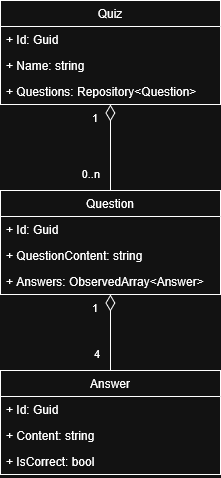
\includegraphics[width=0.2\linewidth]{quiz_uml_simplified.png}
    \centering
    \caption{Uproszczony diagram UML modelu obiektowego aplikacji}
\end{figure}

Relacje między obiektami określiliśmy jako agregację częściową, ponieważ chcieliśmy zezwolić na
tworzenie obiektu ``krok po kroku'', co wymaga istnienia instancji obiektów \verb|Question| oraz
\verb|Answer| poza klasą \verb|Quiz|.

Powyższy diagram przedstawia jednak model w uproszczonej postaci. Pomija bowiem zastosowane przez nas
interfejsy oraz klasy użytkowe, służące łatwiejszemu śledzeniu edycji obiektów. Stworzyliśmy dwie
klasy, \verb|Repository| oraz \verb|ObservedArray|, stanowiące odpowiedniki kolejno słownika oraz
tablicy, implementujące dodatkowo wzorzec obserwatora.

\begin{figure}[H]
    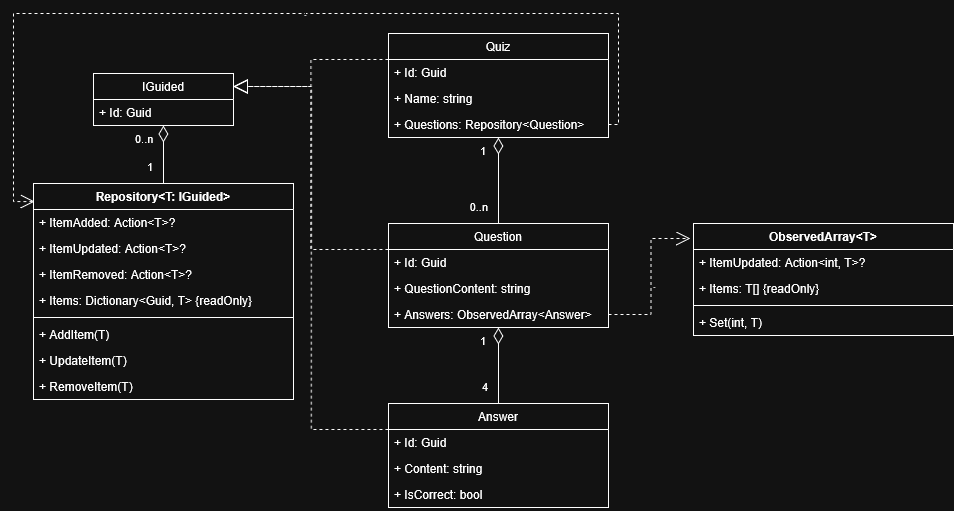
\includegraphics[width=0.75\linewidth]{quiz_uml_full.png}
    \centering
    \caption{Pełny diagram UML modelu obiektowego aplikacji}
\end{figure}

\subsubsection{Serwisy}

W ramach pracy nad generatorem quizów zaimplementowaliśmy dwa serwisy, wykorzystywane
przez wszystkie moduły naszego projektu. Pierwszym z nich jest \verb|QuizSerializer|,
odpowiedzialny za zapis i odczyt quizu z pliku. Wykorzystuje wzorzec strategii, aby
szyfrować serializowane dane. Wspierane obecnie metody szyfrowania to:

\begin{itemize}
    \item Plaintext (brak szyfrowania)
    \item AES
    \item 3DES (Triple DES)
\end{itemize}

\noindent
Dzięki wzorcowi strategii system ten jest jednocześnie silnie rozszerzalny.

Drugim wykorzystywanym przez nas serwisem jest \verb|EncryptionService|. Zaimplementowany
jako singleton, udostępnia gotowe konfiguracje algorytmów AES oraz 3DES. Obecnie inicjalizuje
je za pomocą sztucznych kluczy, w środowisku produkcyjnym należałoby je zamienić na sekrety
aplikacji.

\subsection{Moduł Rozwiązywania Quizu (Mateusz Szymczak)}

Moduł \texttt{QuizSolver\_M} został zrealizowany zgodnie z wzorcem \textbf{MVP (Model-View-Presenter)},
który zapewnia separację logiki biznesowej od interfejsu użytkownika.
Projekt korzysta ze współdzielonych bibliotek \texttt{QuizModel} i \texttt{QuizServices},
zawierających klasy modelu (\texttt{Quiz}, \texttt{Question}, \texttt{Answer})
oraz serwisy serializacji i szyfrowania.

\subsubsection{Architektura MVP}

\begin{itemize}
    \item \textbf{Model} --- klasy \texttt{Quiz}, \texttt{Question}, \texttt{Answer}
          oraz \texttt{QuizSerializer} i \texttt{EncryptionService} współdzielone z generatorem.
    \item \textbf{View (\texttt{SolverView})} --- formularz WinForms implementujący interfejs
          \texttt{ISolverView}. Widok nie zawiera logiki --- wystawia zdarzenia i aktualizuje UI
          na polecenie prezentera.
    \item \textbf{Presenter (\texttt{SolverPresenter})} --- subskrybuje zdarzenia widoku,
          steruje przebiegiem quizu i aktualizuje widok przez metody interfejsu.
\end{itemize}

\subsubsection{Wczytywanie i automatyczne deszyfrowanie}

Po wybraniu pliku przez użytkownika (\texttt{OpenFileDialog}) prezenter próbuje
odszyfrować go kaskadowo, testując kolejno strategie \textbf{AES}, \textbf{TripleDES}
i \textbf{Plaintext}. Dzięki temu aplikacja jest kompatybilna z każdym trybem zapisu
generatora bez konieczności ręcznego wyboru algorytmu.

\begin{lstlisting}
var strategies = new List<IEncryptionStrategy>
{
    EncryptionService.Instance.GetAesStrategy(),
    EncryptionService.Instance.GetTripleDesStrategy(),
    new PlaintextStrategy()
};
foreach (var strategy in strategies)
{
    try
    {
        var serializer = new QuizSerializer(strategy);
        _quiz = serializer.Deserialize(dialog.FileName);
        _questions = _quiz.Questions.Items.Values.ToList();
        _userAnswers = _questions.ToDictionary(
            q => q.Id,
            q => new List<bool> { false, false, false, false });
        _view.SetQuizTitle(_quiz.Name, _questions.Count);
        _view.EnableStart(true);
        return;
    }
    catch { }
}
_view.DisplayError("Nie udalo sie wczytac quizu.");
\end{lstlisting}

\subsubsection{Sterowanie przebiegiem quizu i timer}

Prezenter kontroluje stan interfejsu poprzez włączanie i wyłączanie elementów UI:
\begin{itemize}
    \item \textbf{Po wczytaniu pliku:} aktywowany jest przycisk „Start".
    \item \textbf{Po kliknięciu „Start":} uruchamiany jest \texttt{Timer} (interwał 1000\,ms),
          aktywowane są przyciski nawigacji i „Zakończ".
    \item \textbf{Po kliknięciu „Zakończ":} timer zatrzymywany, checkboxy blokowane,
          obliczany wynik i wyświetlane kolorowe oznaczenia odpowiedzi.
\end{itemize}

\begin{lstlisting}
_timer.Interval = 1000;
_timer.Tick += (s, e) =>
    _view.UpdateTimer((DateTime.Now - _startTime).ToString(@"mm\:ss"));
\end{lstlisting}

\subsubsection{Punktacja i weryfikacja odpowiedzi}

Odpowiedzi użytkownika przechowywane są w słowniku \texttt{\_userAnswers} (klucz: \texttt{Guid} pytania,
wartość: lista 4 wartości \texttt{bool}). Użytkownik otrzymuje 1 punkt za pytanie tylko wtedy,
gdy jego zaznaczenia są identyczne z zestawem poprawnych odpowiedzi (metoda \texttt{SequenceEqual}).

\begin{lstlisting}
private int CalculateScore()
{
    int score = 0;
    foreach (var q in _questions)
    {
        var correct = q.Answers.Items.Select(a => a.IsCorrect).ToList();
        var user = _userAnswers[q.Id];
        if (correct.SequenceEqual(user)) score++;
    }
    return score;
}
\end{lstlisting}

\subsubsection{Podgląd poprawnych i błędnych odpowiedzi}

Po zakończeniu quizu użytkownik może przeglądać pytania z oznaczeniem kolorystycznym odpowiedzi:
\begin{itemize}
    \item \textcolor{green!60!black}{\textbf{Zielony}} --- zaznaczona i poprawna,
    \item \textcolor{orange}{\textbf{Pomarańczowy}} --- poprawna, ale niezaznaczona (pominięta),
    \item \textcolor{red}{\textbf{Czerwony}} --- zaznaczona, ale błędna.
\end{itemize}

Checkboxy pozostają wizualnie włączone (WinForms przy \texttt{Enabled = false} nadpisuje
\texttt{ForeColor} na szary, co uniemożliwiałoby wyświetlenie kolorów), a blokada zmian
realizowana jest przez flagę \texttt{\_quizEnded} w presenterze.

\begin{lstlisting}
private void OnEndQuiz()
{
    _timer.Stop();
    _elapsed = DateTime.Now - _startTime;
    _quizEnded = true;
    _view.EnableEnd(false);
    _view.EnableNavigation(true);
    int score = CalculateScore();
    ShowCorrectAnswers();
    _view.ShowResult(score, _questions.Count, _elapsed);
}
\end{lstlisting}


\subsection{Moduł Generatora Quizu (Dawid Piotrowski)}

Moduł generatora quizów został zrealizowany w oparciu o architekturę trójwarstwową przy użyciu wzorca projektowego \textbf{MVP (Model-View-Presenter)}. Odpowiada on za zarządzanie listą dostępnych testów, tworzenie i edycję pytań oraz bezpieczny zapis i odczyt danych przy użyciu dedykowanych interfejsów kryptograficznych.

\subsubsection{Architektura panelu zarządzania quizami}

Główny punkt wejścia modułu administracyjnego stanowi panel listy quizów. Zaimplementowano go z zachowaniem pełnej separacji odpowiedzialności pomiędzy poszczególnymi warstwami:

\begin{itemize}
    \item \textbf{Model} --- reprezentowany przez generyczną klasę \texttt{Repository<Quiz>} (współdzieloną ze słownika modelu).
    \item \textbf{View (\texttt{QuizListView})} --- klasa widoku implementująca interfejs \texttt{IQuizListView}. Warstwa ta odpowiada wyłącznie za renderowanie kontrolek interfejsu oraz przechwytywanie akcji użytkownika, które są przekazywane za pomocą zdarzeń do prezentera.
    \item \textbf{Presenter (\texttt{QuizListPresenter})} --- komponent pośredniczący, który subskrybuje zdarzenia widoku (\texttt{AddQuiz}, \texttt{OpenQuiz}, \texttt{LoadQuiz}) oraz reaguje na modyfikacje danych w modelu (\texttt{ItemAdded}, \texttt{ItemUpdated}, \texttt{ItemRemoved}), automatycznie synchronizując stan interfejsu graficznego.
\end{itemize}

\subsubsection{Mechanizm dynamicznej synchronizacji widoku}

W celu zachowania pełnej reaktywności interfejsu, prezenter wiąże zdarzenia zmiany kolekcji repozytorium z delegatem aktualizującym kontrolki widoku. Wykorzystanie mapowania obiektów domenowych za pomocą obiektu typu data transfer object (DTO) pozwala na uniezależnienie widoku od modelu:

\begin{lstlisting}[caption={Konstruktor prezentera listy quizów i rejestracja zdarzeń}]
public QuizListPresenter(IQuizListView view, Repository<Quiz> quizList)
{
    this.view = view;
    this.quizList = quizList;

    Action<Quiz> updateQuizList = quiz => this.view.UpdateQuizList(this.quizList.Items.Values.Select(QuizToDto));
    this.quizList.ItemAdded += updateQuizList;
    this.quizList.ItemUpdated += updateQuizList;
    this.quizList.ItemRemoved += updateQuizList;

    this.view.AddQuiz += () => OpenQuizForm(null);
    this.view.OpenQuiz += OpenQuizFormForEdition;
    this.view.LoadQuiz += LoadQuiz;
}
\end{lstlisting}

\subsubsection{Architektura formularza zarządzania pojedynczym quizem}

Formularz pojedynczego quizu odpowiada za modyfikację nazwy testu, zarządzanie powiązaną z nim kolekcją pytań oraz operacje utrwalania danych na dysku. Logika została zaimplementowana z zachowaniem ścisłego podziału warstw:

\begin{itemize}
    \item \textbf{Model} --- reprezentowany przez klasę domenową \texttt{Quiz} (zawierającą wewnętrzne repozytorium pytań).
    \item \textbf{View (\texttt{SingleQuizView})} --- klasa formularza implementująca interfejs \texttt{ISingleQuizView}. Odpowiada za prezentację danych dotyczących quizu oraz przełączanie między trybem tworzenia lub edycji za pomocą dedykowanej metody \texttt{EnableEdition}. Wszystkie interakcje użytkownika są mapowane bezpośrednio na zdarzenia interfejsu.
    \item \textbf{Presenter (\texttt{SingleQuizPresenter})} --- komponent zarządzający cyklem życia formularza. Inicjalizuje stan widoku w zależności od kontekstu wywołania (tryb tworzenia nowej instancji lub edycji istniejącej), subskrybuje zdarzenia interfejsu użytkownika oraz reaguje na zmiany w obserwowalnej kolekcji pytań modelu, wymuszając automatyczne odświeżenie widoku.
\end{itemize}

\subsubsection{Walidacja danych}

W celu zapewnienia poprawności struktur danych przed wykonaniem operacji zapisu lub modyfikacji, prezenter wykorzystuje wewnętrzną klasę narzędziową \texttt{QuizValidator}. Implementuje ona minimalne wymagania dla struktury testu:

\begin{itemize}
    \item \textbf{Niepusta nazwa:} Nazwa quizu musi być niepusta i nie składać się tylko z białych znaków
    \item \textbf{Niepusta zawartość:} W quizie musi pojawić się przynajmniej jedno pytanie
\end{itemize}

\subsubsection{Serializacja quizu}

Wykorzystując wzorzec strategii oraz singleton, program zapisuje dane quizu na dysk za pośrednictwem usługi \verb|QuizSerializer|.

\begin{lstlisting}[caption={Serializacja quizu}]
IEncryptionStrategy strategy = encryptionStrategy switch
{
    EncryptionStrategyDto.Plaintext => new PlaintextStrategy(),
    EncryptionStrategyDto.Aes => EncryptionService.Instance.GetAesStrategy(),
    EncryptionStrategyDto.TripleDes => EncryptionService.Instance.GetTripleDesStrategy(),
    _ => throw new ArgumentOutOfRangeException(nameof(encryptionStrategy), encryptionStrategy, null)
};

var serializer = new QuizSerializer(strategy);
var validator = new QuizValidator();

var error = validator.ValidateQuiz(this.quiz);
if (error == null)
{
    try
    {
        serializer.Serialize(this.quiz, quizFilePath);
    }
    catch(CryptographicException)
    {
        this.view.DisplayError("Zapisanie quizu do pliku nie powiodlo sie :(");
    }
}
else
{
    this.view.DisplayError(error);
}
\end{lstlisting}

\subsubsection{Architektura formularza zarządzania pojedynczym pytaniem}

Formularz pojedynczego pytania odpowiada za definiowanie treści pytania testowego oraz zarządzanie powiązanym zestawem dokładnie czterech wariantów odpowiedzi. Logika została zaimplementowana z zachowaniem pełnej separacji odpowiedzialności pomiędzy warstwami:

\begin{itemize}
    \item \textbf{Model} --- reprezentowany przez klasę domenową \texttt{Question} (zawierającą wewnętrzne repozytorium obiektów \texttt{Answer}).
    \item \textbf{View (\texttt{SingleQuestionView})} --- klasa formularza implementująca interfejs \texttt{ISingleQuestionView}. Odpowiada za prezentację danych pytania oraz przełączanie między trybem dodawania pytania i jego edycji. Widok wykorzystuje także mechanizm \verb|UserControl| w WinForms'ach, aby stworzyć osobną kontrolkę do wprowadzania odpowiedzi na pytania.
    \item \textbf{Presenter (\texttt{SingleQuestionPresenter})} --- komponent pośredniczący, który inicjalizuje stan kontrolek (w trybie dodawania nowej pozycji lub edycji istniejącej), subskrybuje zdarzenia widoku i konstruuje obiekt przed ostatecznym zatwierdzeniem.
\end{itemize}

\subsubsection{Walidacja danych}

W celu zapewnienia integralności danych przed zapisem lub modyfikacją pytania wewnątrz struktury quizu, prezenter wykorzystuje pomocniczą klasę \texttt{QuestionValidator}. Odpowiada ona za walidację:

\begin{itemize}
    \item \textbf{Niepusta treść:} Treść pytania nie może być pusta
    \item \textbf{Cztery niepuste odpowiedzi:} Odpowiedzi nie mogą być puste
    \item \textbf{Co najmniej jedna odpowiedź poprawna:} Co najmniej jedna z odpowiedzi musi być oznaczona jako poprawna
\end{itemize}

\subsubsection{Mechanizm obsługi zdarzeń i synchronizacji stanu kontrolki użytkownika}

W celu zachowania pełnej reaktywności interfejsu bez wprowadzania ścisłego powiązania warstw, konstruktor widoku wiąże wewnętrzne delegaty zdarzeń kontrolek \texttt{SingleAnswer} z potokiem zdarzeń prezentera, przekazując indeks modyfikowanej odpowiedzi:

\begin{lstlisting}[caption={Inicjalizacja kontrolek użytkownika i rejestracja zdarzeń w SingleQuestionView}]
public SingleQuestionView()
{
    InitializeComponent();

    answerForms = new SingleAnswer[] { ans1, ans2, ans3, ans4 };

    for (int i = 0; i < answerForms.Length; i++)
    {
        var index = i;
        answerForms[index].TextChanged += (sender, e) =>
        {
            AnswerUpdated?.Invoke(index, new AnswerDto(answerForms[index].AnswerContent, answerForms[index].IsCorrect));
        };
        answerForms[index].IsCorrectChanged += (sender, e) =>
        {
            AnswerUpdated?.Invoke(index, new AnswerDto(answerForms[index].AnswerContent, answerForms[index].IsCorrect));
        };
    }
}
\end{lstlisting}

\subsection{Alternatywny Moduł Rozwiązania Quizu (Filip Kłos)}

Druga aplikacja, \texttt{QuizSolver}, służy do wczytywania i rozwiązywania quizów utworzonych w głównym generatorze. Aby zachować spójność kodu i uniknąć jego duplikacji, projekt wykorzystuje wspólne biblioteki klas: \texttt{QuizModel} (zawierającą definicje struktur danych) oraz \texttt{QuizServices} (odpowiadającą za logikę serializacji i kryptografii).

\subsubsection{Architektura MVP}
Architektura aplikacji opiera się na wzorcu projektowym \textbf{Model-View-Presenter (MVP)}.
\begin{itemize}
    \item \textbf{Model} --- wykorzystuje klasy domenowe takie jak \texttt{Quiz} oraz \texttt{Question} pochodzące ze współdzielonej biblioteki.
    \item \textbf{View} --- opiera się na interfejsach, takich jak \texttt{ISingleQuestionView} oraz \texttt{IFileReaderView}, które są implementowane przez formularze WinForms. Widoki pełnią rolę pasywną i przekazują akcje użytkownika bezpośrednio do warstwy prezentera.
    \item \textbf{Presenter} --- klasy takie jak \texttt{QuizSolverPresenter} subskrybują zdarzenia widoku, sterują przepływem aplikacji i zliczają punkty na koniec quizu.
\end{itemize}

\subsubsection{Wczytywanie i obsługa strategii z poziomu interfejsu}
Widok \texttt{FileReaderView} umożliwia użytkownikowi wybór pliku oraz odpowiednich strategii (szyfrowania i punktacji) z rozwijanych list. Wybrane parametry trafiają do klasy \texttt{FileReaderPresenter}, która na ich podstawie tworzy odpowiednie obiekty i uruchamia główne okno quizu.

\begin{lstlisting}[caption={Wybór strategii oceniania i uruchomienie quizu w FileReaderPresenter}]
IScoringStrategy scoringStrategy = scoringStrategyName switch
{
    "Rygorystyczne" => new StrictScoringStrategy(),
    "Częściowe" => new PartialScoringStrategy(),
    _ => new StrictScoringStrategy()
};

var quizSolverPresenter = new QuizSolverPresenter(quizSolverView, loadedQuiz, scoringStrategy);
\end{lstlisting}

\subsubsection{Obsługa pytań wielokrotnego wyboru}
Aplikacja zastępuje klasyczne kontrolki jednokrotnego wyboru komponentami typu \texttt{CheckBox}. Rozwiązanie to pozwala na zaznaczenie wielu poprawnych odpowiedzi w ramach jednego pytania. Zebrane indeksy zaznaczonych odpowiedzi są przesyłane do prezentera za pomocą dedykowanego zdarzenia \texttt{AnswerSubmitted}.

\begin{lstlisting}[caption={Zbieranie odpowiedzi z kontrolek CheckBox w widoku}]
List<int> selectedIndices = new List<int>();

if (cbAnswer0.Checked) selectedIndices.Add(0);
if (cbAnswer1.Checked) selectedIndices.Add(1);
if (cbAnswer2.Checked) selectedIndices.Add(2);
if (cbAnswer3.Checked) selectedIndices.Add(3);

AnswerSubmitted?.Invoke(selectedIndices);
\end{lstlisting}

\subsubsection{Wzorzec Strategii w mechanizmie oceniania}
W celu zapewnienia dużej elastyczności w sposobie obliczania punktów, w logice oceniającej zastosowano wzorzec \textbf{Strategia (Strategy Pattern)}. Zdefiniowano interfejs \texttt{IScoringStrategy} oraz dwie konkretne implementacje:

\begin{enumerate}
    \item \textbf{\texttt{StrictScoringStrategy} (Ocenianie rygorystyczne)} -- Przyznaje jeden punkt tylko w sytuacji, gdy użytkownik zaznaczy wszystkie poprawne odpowiedzi i nie zaznaczy żadnej odpowiedzi błędnej. Weryfikacja opiera się na metodach rozszerzających dostarczanych przez bibliotekę LINQ.
    \item \textbf{\texttt{PartialScoringStrategy} (Ocenianie częściowe)} -- Przydziela punkty dodatnie za każdą poprawnie zaznaczoną odpowiedź, ale jednocześnie odejmuje punkty za zaznaczenie opcji błędnej, pilnując, aby końcowy wynik dla danego pytania nie przyjął wartości ujemnej.
\end{enumerate}

\begin{lstlisting}[caption={Implementacja rygorystycznego zliczania punktów przy użyciu LINQ}]
// Sprawdzenie idealnego dopasowania zaznaczonych odpowiedzi
bool isCorrect = (correctIndices.Count == selectedIndices.Count) &&
                 !correctIndices.Except(selectedIndices).Any();

return isCorrect ? 1 : 0;
\end{lstlisting}

\section{Wnioski}
\begin{itemize}
    \item \textbf{Spostrzeżenia:} Zastosowanie wzorca projektowego MVP w aplikacji Windows Forms znacząco ułatwiło separację logiki od interfejsu graficznego.
    \item \textbf{Osiągnięcia:} Zrealizowano poprawnie funkcjonującą warstwę prezentera oraz szyfrowanie/deszyfrowanie plików projektowych.
    \item \textbf{Potencjał rozwoju:} Aplikację można w przyszłości rozbudować o możliwość eksportu statystyk do bazy danych, czy obsługę multimediów w pytaniach.
\end{itemize}

\section{Bibliografia}
\begin{enumerate}
    \item Wytyczne do zadania nr 4 - ,,Quiz''
    \item Dokumentacja języka C\# i platformy .NET
    \item Wykład ,,Diagramy UML''
\end{enumerate}

\end{document}